\documentclass{beamer}

\usepackage[spanish,activeacute,es-tabla]{babel}
\usepackage[utf8]{inputenc} % mac utf8
%\usepackage{beamerthemesplit}
\usepackage{array}
\spanishdecimal{.}

\usepackage{pgfplots}
\pgfplotsset{compat=1.18}
\usepackage{graphicx}
\DeclareGraphicsExtensions{.png,.pdf,.jpg}


\usefonttheme{professionalfonts} % fuentes de LaTeX 
\usetheme{Boadilla}	% tema escogido en este ejemplo 




\setbeamertemplate{caption}[numbered]

\newtheorem{Teorema}{Teorema} 
\newtheorem{Ejemplo}{Ejemplo} 
\newtheorem{Definicion}{Definici\’on} 
\newtheorem{Corolario}{Corolario} 
\newtheorem{Prueba}{Prueba}

\newtheorem{teorema} [Teorema] {Teorema}
\newtheorem{ejemplo} [Ejemplo] {Ejemplo}
\newtheorem{definicion} [Definicion]{Definición} 
\newtheorem{ejercicio} [Corolario]{Ejercicio} 
\newtheorem{lema} [theorem] {Lema}

\setbeamertemplate{theorems}[numbered] 





\title[]{Tema 3. Codificación económica}
\author[José A Montenegro (jmmontes@uma.es)]{José A. Montenegro}
\institute{Dpto. Lenguajes y Ciencias de la Computación\\
ETSI Informática. Universidad de Málaga\\
jmmontes@uma.es
%\href{https://twitter.com//monteDocencia}{
%
\includegraphics[height=0.03\textheight]{twitter.jpg}}
}
\date{\today}

%###########################################################################
% FootLine
%###########################################################################

\setbeamertemplate{footline} {%
\leavevmode%
  \hbox{\begin{beamercolorbox}[wd=.5\paperwidth,ht=2.5ex,dp=1.125ex,leftskip=.3cm plus1fill,rightskip=.3cm]{author in head/foot}%
    \usebeamerfont{author in head/foot}\insertshortauthor 
  \end{beamercolorbox}%
  
  \begin{beamercolorbox}[wd=.5\paperwidth,ht=2.5ex,dp=1.125ex,leftskip=.3cm,rightskip=.3cm plus1fil]{title in head/foot}%
    Teoría de la Información y Codificación \hfill    \insertpagenumber /\insertdocumentendpage
  \end{beamercolorbox}}%
  \vskip0pt%
}%

%###########################################################################
% Document
%###########################################################################

\begin{document}

%\setbeamertemplate{headline}[title slide]
%\setbeamertemplate{footline}[title slide]


%###########################################################################
% Tíitulo
%###########################################################################
\begin{frame}

\includegraphics[height=0.15\textheight]{logoUma.jpg} \hspace*{3.5cm}

\includegraphics[height=0.17\textheight]{logoInf.jpg}   \hspace*{3.5cm}

\includegraphics[height=0.17\textheight]{logoLcc.jpg}  

\titlepage


\setbeamertemplate{footline}[body]
\setbeamertemplate{headline}[body]
\end{frame}

%###########################################################################
% Contenidos
%###########################################################################

\section[Resumen]{}
\frame{\tableofcontents}

\section{El concepto de fuente}% The concept of a source}

\begin{frame} \frametitle{El concepto de fuente}     \small
 
\begin{itemize}

\item Básicamente podemos definir como una ``\textbf{fuente}'' como un productor de mensajes. 

	\begin{itemize}
		\item Los ejemplos de la vida real van desde un persona escribiendo correos, o un escáner digitalizando imágenes. 
	\end{itemize}

\item Utilizando la terminología anteriormente descrita, una fuente emite una cadena de símbolos, denotado por:

\begin{center}$\xi_1 \xi_2 \xi_3 \ldots .$\end{center}

Cada $\xi_k$ es una variable que puede tomar como valor cualquier símbolo que pertenece a un alfabeto dado.


\end{itemize}



\end{frame}


%%%%%%%%%%%%%%%%%%


\begin{frame}      \small

\begin{itemize}
\item Una característica que define una fuente y la diferencia de otra es el alfabeto. 
 
     \begin{itemize}
    	  \item Idiomas orientales utilizan alfabetos distintos al alfabeto de 28 letras $\mathbb{A}$. 
     \end{itemize}
 
\item Muchos comparten el alfabeto de 28-27 letras similar a $\mathbb{A}$, existen ciertas reglas de como el alfabeto es utilizado (gramática, sintaxis ...) y esos elementos están reflejados en la cadena emitida por la fuente.

\begin{itemize}
 
\item El símbolo W aparece mucho más en el Inglés que en otro idioma. 

 \item Escáner o Fax, producirá más a menudo mensajes en el que W (representa un pixel blanco)  que B (representa un pixel negro). 
 \item Compresión Fax:

        \begin{itemize}
         \item  \url{https://en.wikipedia.org/wiki/Modified\_Huffman\_coding}
         \item  \url{https://en.wikipedia.org/wiki/Fax#Compression}
         \end{itemize}
\end{itemize}
\end{itemize}
\end{frame}


\subsection{Ejemplos}

%%%%%%%%%%%%%%%%%%%%%%%%%%%%%%%%
\begin{frame}\frametitle{Ejemplos Lenguajes Naturales} \footnotesize
\begin{itemize}
\item  Como conclusión tenemos que la fuente debe ser descrita especificando el alfabeto y las probabilidades de los símbolos que van a ser emitidos.
\end{itemize}
 
\tiny
\begin{table}
\center
\begin{tabular}{|c||c|c|c|c|}
\hline
Símbolo	&	Español	&	Portugues	&	Italiano	&	Inglés	\\
a 	&	12.53\% 	&	14.63\% 	&	11.74\% 	&	8,167\%	\\
b 	&	1.42\% 	&	1.04\% 	&	0.92\% 	&	1,492\%	\\
c 	&	4.68\% 	&	3.88\% 	&	4.5\% 	&	2,782\%	\\
d 	&	5.86\% 	&	4.99\% 	&	3.73\% 	&	4,253\%	\\
e 	&	13.68\% 	&	12.57\% 	&	11.79\% 	&	12,702\%	\\
f 	&	0.69\% 	&	1.02\% 	&	0.95\% 	&	2,228\%	\\
g 	&	1.01\% 	&	1.30\% 	&	1.64\% 	&	2,015\%	\\
h 	&	0.70\% 	&	1.28\% 	&	1.54\% 	&	6,094\%	\\
i 	&	6.25\% 	&	6.18\% 	&	11.28\% 	&	6,966\%	\\
j 	&	0.44\% 	&	0.40\% 	&	0.00\% 	&	0,153\%	\\
k 	&	0.01\% 	&	0.02\% 	&	0.00\% 	&	0,772\%	\\
$\ldots$ 	&	$\ldots$ 	&	$\ldots$ 	&	$\ldots$ 	&	$\ldots$	\\
q 	&	0.88\% 	&	1.20\% 	&	0.51\% 	&	0,095\%	\\
r 	&	6.87\% 	&	6.53\% 	&	6.37\% 	&	5,987\%	\\
s 	&	7.98\% 	&	7.81\% 	&	4.98\% 	&	6,327\%	\\
t 	&	4.63\% 	&	4.74\% 	&	5.62\% 	&	9,056\%	\\
u 	&	3.93\% 	&	4.63\% 	&	3.01\% 	&	2,758\%	\\
v 	&	0.90\% 	&	1.67\% 	&	2.10\% 	&	0,978\%	\\
w 	&	0.02\% 	&	0.01\% 	&	0.00\% 	&	2,36\%	\\
x 	&	0.22\% 	&	0.21\% 	&	0.00\% 	&	0,15\%	\\
y 	&	0.90\% 	&	0.01\% 	&	0.00\% 	&	1,974\%	\\
z 	&	0.52\% 	&	0.47\% 	&	0.49\% 	&	0,074\%\\
\hline
\end{tabular}
\end{table}



\end{frame} 

%%%%%%%%%%%%%%%%%%%%%%%%%%%%%%%%


\begin{frame}\frametitle{Ejemplos Moneda}      \small

 \begin{itemize}

 \item  Experimento de una moneda es lanzada repetidamente, resultado $H = Cara$, $T = Cruz$. Una fuente con alfabeto S = \{H,T\}

 \item Si la moneda no está trucada, la cadena emitida podría ser

\begin{center}
$HTTHTHTHTTHHTTTHTHHTTHTHTHTH \ldots$,
\end{center}

donde H y T ocurren con la misma frecuencia. 

 \item La probabilidad que $\xi_k$ sea H y la probabilidad que $\xi_k$ sea T, es la misma $1/2$. Lo representaríamos como:
\begin{center}
$Pr(\xi_k =H) = Pr(\xi_k =T)=0.5$
\end{center}

 \item Por otro lado, una moneda trucada podría emitir un cadena como :
\begin{center}
$HHHHHHHTHHHHHTHHHHHHHHHHT \ldots$
\end{center}

donde las probabilidades son tales que $Pr(\xi_k =H)$ es significativamente mayores que $Pr(\xi_k =T)$.

\end{itemize}
\end{frame}

%%%%%%%%%%%%%%%%%%

\subsection{Distribución de Probabilidad}
\begin{frame} \frametitle{Distribución de Probabilidad}     \small
 
 
 La teoría necesaria para establecer un modelo matemático completo de la fuente, es bastante complejo pero podemos realizar algunos progresos basándonos en un modelo simple.


\begin{definicion}[Distribución de Probabilidad]
Sea  $S =\{s_1, s_2, . . . , s_m\}$ un alfabeto. Una distribución de probabilidad sobre S es un conjunto de números reales $p_1,p_2,...,p_m$ tal que 
\begin{center}
$p_1 +p_2 + ... +p_m =1, \;\;\;	0\leq p_i \leq 1 (i=1,2,...,m)$
\end{center}

Las probabilidades pueden ser descritas como un vector  $\mathbf{p} = [p_1, p_2, . . . , p_m]$, y establece la relación que el símbolo $s_i$ aparece con probabilidad $p_i$.
\end{definicion}


\end{frame}

%%%%%%%%%%%%%%%%%%

\subsection{Fuente con probabilidad de distribución}
\begin{frame}\frametitle{Fuente con probabilidad de distribución}      \small

\begin{itemize}
\item Dada una distribución de probabilidad \textbf{p} en \textit{S}, consideramos una fuente con la siguiente propiedad:

\begin{itemize}
\item La fuente emite una cadena $\xi_1 \xi_2 \xi_3 \ldots $, donde el valor de cada $\xi_k$ es un miembro del alfabeto \textit{S}, y para toda k, la probabilidad que $\xi_k$ tome un valor determinado $s_i$ es dado por la ecuación:

\begin{center}
$Pr(\xi_k =s_i)=p_i$
\end{center}

\item Donde $\xi_k$ es una \textit{variable aleatoria}.

\end{itemize}


\item  Nos referimos a este modelo como una ``fuente con probabilidad de distribución \textbf{p}'' o simplemente una ``fuente (S,\textbf{p})'' . 

\item  Esta definición no implica que todas las características de la fuente son descritas mediante \textbf{p}. Representa que la probabilidad de distribución para cada $\xi_k$ es la misma.
\end{itemize}


\end{frame}

%%%%%%%%%%%%%%%%%%

\begin{frame}      \small

\begin{itemize}
\item En muchos casos esta es una suposición razonable, aunque la fuente puede tener otras características. 
 

\begin{itemize}
\item Por ejemplo, suponemos que el texto de un libro es una cadena de símbolos del alfabeto $\mathbb{A}$. 

\item Si abrimos el libro en la página $x$ y buscamos el $y$ ésimo símbolo en esa página, entonces la probabilidad que el símbolo sea $L$ puede ser asumido que es la misma, para toda $x$ e $y$.

\item Pero si sabemos que la letra 17 en la página 83 es una $L$, entonces afectará a la probabilidad que la letra 18 de la página 83 sea una $A$. 
\end{itemize}

\item Imponiendo que las variables aleatorias $\xi_k$  tienen la misma distribución \textbf{p}, pero en general, no asumimos que esas variables aleatorias son $independientes$.
\end{itemize}

\end{frame}
%%%%%%%%%%%%%%%%%%
\subsection{Fuente sin memoria}
\begin{frame}  \frametitle{Fuente sin memoria}    \small
\begin{definicion}[Fuente sin memoria]
Una fuente (S,\textbf{p}) que emite una cadena $\xi_1 \xi_2 \xi_3 \ldots $ es sin memoria si las variables aleatorias $\xi_k$ son independientes. O lo que es lo mismo, para todos \textit{k} y \textit{l}

\begin{center}
$Pr(\xi_k =s_i$ y $\xi_l =s_j)$ = $\;Pr(\xi_k =s_i) *  Pr(\xi_l =s_j)$
\end{center}
\end{definicion}

\begin{itemize}
\item  En una fuente sin memoria, el conocimiento de algunas partes del mensaje no afecta a la distribuciones de probabilidades asignadas a los otros términos. 

\item Esta situación ocurre en el experimento realizado al lanzar una moneda al aire y otras situaciones en la vida real.
\end{itemize}

\end{frame}

%%%%%%%%%%%%%%%%%%

\subsection{Ejemplos y Ejercicios}

\begin{frame}  \frametitle{Ejemplos}    \small
 
 \begin{ejemplo}
Una de las apuestas más conocidas en España es la quiniela, que puede ser representada como una fuente que emite una cadena de símbolos del alfabeto S = \{1,x,2\}, donde 1 = gana casa, x = empate, 2 = gana foráneo. ¿Podría ser considerado este ejemplo como una fuente sin memoria?
\end{ejemplo}

\pause
\textit{\underline{Solución}}:\\
 Es razonable asumir que la fuente es sin memoria, ya que el resultado de un partido de fútbol no afecta al resultado de los otros partidos. Un estudio en los resultados obtenidos es que la probabilidad de distribución es aproximadamente:

\begin{center}
$p_1 = 0.42,	p_x = 0.26,	p_2 = 0.31.$
\end{center}

%\todo{(the Bayesian approach).}

\end{frame}



%%%%%%%%%%%%%%%%%%%%%%%%%%%%%%%%
\begin{frame}  \small

\begin{ejercicio} Considere una fuente que emite símbolos del alfabeto S con probabilidad de distribución p, donde 
$S = \{a,b,c\}$	  $p = [p_a,p_b,p_c] =$ [0.6,0.3,0.1].

Si la fuente emite una cadena de 100 símbolos, aproximadamente ¿Cuántas veces aparecerá el carácter a?  Si la fuente es sin memoria, aproximadamente ¿Cuántas veces aparecerá el par ab ?
\end{ejercicio}
\pause
\textit{\underline{Solución}}:\\
a) 60, b)18




\end{frame} 

%%%%%%%%%%%%%%%%%%%%%%%%%%%%%%%%
%%%%%%%%%%%%%%%%%%%%%%%%%%%%%%%%
%%%% SECCION
%%%%%%%%%%%%%%%%%%%%%%%%%%%%%%%%
%%%%%%%%%%%%%%%%%%%%%%%%%%%%%%%%
%%%%%%%%%%%%%%%%%%%%%%%%%%%%%%%%

\section{El problema de optimización}
%%%%%%%%%%%%%%%%%%%%%%%%%%%%%%%%

\begin{frame}  \small \frametitle{El problema de optimización}

\begin{itemize}
\item Consideremos que ocurre cuando la fuente (S,p) emite una cadena y es transformada a una cadena codificada utilizando un alfabeto \textit{T}. 

\begin{itemize}
\item ¿En que grado depende la longitud de un mensaje del código utilizado $c: S\rightarrow T^{*}$?
\end{itemize}

\item Partimos $S = \{s_1, s_2, \ldots , s_m\}$.  

\begin{itemize}
\item Sea $y_i$ la \underline{longitud de la palabra codificada} $c(s_i) (1\leq i \leq m)$, y consideramos un mensaje en S de longitud \underline{N}. 
\item Si N es un número razonadamente grande, el mensaje contendrá el símbolo $s_1$ aproximadamente $Np_1$ veces, $s_2$ unas $Np_2$ veces $\ldots$. 

\item Después de codificar aplicando la función $c$,  tendremos $Np_1$  cadenas $c(s_1)$, cada una de longitud $y_1$,  $Np_2$  cadenas $c(s_2)$, cada una de longitud $y_2$ y así con todas.
\end{itemize}



\end{itemize}

\end{frame} 

\subsection{Longitud media de palabras}

%%%%%%%%%%%%%%%%%%%%%%%%%%%%%%%%
\begin{frame} \frametitle{Longitud media de palabras} \small

\begin{itemize}

\item  La \underline{longitud total del mensaje} codificado es aproximadamente:


\begin{center}
$Np_1y_1 + Np_2y_2 + \ldots Np_my_m	= N(p_1y_1 + p_2y_2 + \ldots + p_my_m).$
\end{center}

\item Por tanto, si el \underline{mensaje original} tiene longitud \underline{N}, el \underline{mensaje codificado} tiene una longitud de \underline{LN}, donde:
\begin{center}
$L=p_1y_1+p_2y_2+ \ldots +p_my_m$.
\end{center}

\end{itemize}

\begin{definicion}[Longitud media de palabras]
La longitud media de palabras de un código $c: S\rightarrow T^{*}$ para la fuente $(S, \mathbf{p})$ es 

\begin{center}$L=p_1y_1+p_2y_2+ \ldots +p_my_m$.\end{center}

\end{definicion}




\end{frame} 
%%%%%%%%%%%%%%%%%%%%%%%%%%%%%%%%
\begin{frame}  \small

\begin{ejemplo}

Sea $S=\{s_1,s_2,s_3\}$ y p = [0.2, 0.6, 0.2]. Debemos encontrar el valor de L cuando utilizamos el código binario:
\begin{center} $s_{1}  \mapsto 0, s_{2}  \mapsto 10, s_{3}  \mapsto 11$\end{center}
Además, ¿Es el código binario asignado para S el que alcanza su menor valor?
\end{ejemplo}

\pause

\underline{\textit{Solución}}:\\

 El valor de L es: 1 x 0.2 + 2 x 0.6 + 2 x 0.2 = 1.8.

Ya que $s_2$ es el símbolo más utilizado, podríamos dar una codificación que utilice la palabra codificada más corta para este símbolo, tal que 
\begin{center} $s_{1}  \mapsto 10, s_{2}  \mapsto 0, s_{3}  \mapsto 11$\end{center}
		
Donde el valor de L es: 2 x 0.2 + 1 x 0.6 + 2 x 0.2 = 1.4. 

\end{frame} 

\subsection{Código Optimo}
%%%%%%%%%%%%%%%%%%%%%%%%%%%%%%%%
\begin{frame} \frametitle{Código Optimo} \small

\begin{itemize}
\item En el ejemplo anterior ha sido fácil probar que existe un código mejor que el original, pero tenemos un problema mayor que resolver. 

\item Dado una fuente (S,\textbf{p}) y el alfabeto T, ¿Cómo podemos encontrar un código $c: S\rightarrow T^{*}$ para el cual L es el mínimo posible?

\end{itemize}

\begin{definicion}[Código optimo]
Dado una fuente (S,\textbf{p}) y un alfabeto T, un código UD $c: S\rightarrow T^{*}$  es óptimo si no existe un código con longitud media de palabra menor.
\end{definicion}

\begin{itemize}
\item El requisito que un código sea UD es una restricción significativa.  

\item En el tema anterior mostramos que esta restricción puede ser expresada por la condición $K\leq 1$, donde K es el número  Kraft-McMillan asociado con los parámetros $n_1,n_2,...,n_M$ y la base b del código: 
\begin{center}
    $K=n_1/b +n_2/b^2 + \ldots +n_M / b^M$ 
\end{center}

\end{itemize}

\end{frame} 

%%%%%%%%%%%%%%%%%%%%%%%%%%%%%%%%
\begin{frame}  \small

\begin{itemize}
\item  En nuestra notación, $n_i$ es el número de símbolos $s_j$ tal que $y_j=i$, y M es el máximo valor de $y_j$. 

\item El término $\frac{n_i}{b^ i}$ en K es la suma de $n_i$ términos $\frac{1}{b^ i}$, correspondientes a un término $\frac{1}{b^{y_j}}$ para cada j tal que  $y_j = i$.


\item De esta forma K puede ser escrito como la suma de todos los términos $\frac{1}{b^{y_j}}$:

\begin{center}$K=\frac{1}{b^{y_1}}+\frac{1}{b^{y_2}}+ \ldots +\frac{1}{b^{y_m}}$ \end{center}


\item Reescribiendo la condición $K\leq 1$ en esta forma podemos formular el problema de encontrar los códigos óptimos como sigue:
\vspace{0.5cm}
\begin{itemize}
\item Dado b y $p_1,p_2, \ldots, p_m$ encontrar  $y_1,y_2,\ldots,y_m$ que:
\vspace{0.5cm}
\begin{center}minimizar  $p_1y_1 + p_2y_2 + \ldots + p_my_m$\end{center}
\begin{center}sujeto a $\frac{1}{b^{y_1}}+\frac{1}{b^{y_2}}+ \ldots +\frac{1}{b^{y_m}} \leq 1$.\\
$y_1,y_2,\ldots,y_m \geq 0$ 
\end{center}
\end{itemize}

\end{itemize}

\end{frame} 

%%%%%%%%%%%%%%%%%%%%%%%%%%%%%%%%
\begin{frame}  \small

\begin{ejercicio}
Una fuente emite tres símbolos con probabilidades 0.5, 0.25, 0.25. Construya un código binario PF para esta fuente con un tamaño medio de palabra de 1.5.\\
\end{ejercicio}

\pause

\underline{\textit{{Solución}}}:\\

Por ejemplo: $s_1 \mapsto 0, s_2 \mapsto 10, s_3 \mapsto 11$
 \begin{center}
L = 1x0,5 + 2 x 0,25 + 2 x 0,25  =1,5
\end{center}

\end{frame} 

%%%%%%%%%%%%%%%%%%%%%%%%%%%%%%%%
\section{Entropía e Incertidumbre}


\begin{frame} \frametitle{Entropía} \small

\begin{definicion}[Entropía de una distribución]

La entropía base b de una distribución de probabilidad $p = [p_1, p_2, . . . , p_m]$ es 

\begin{center}
$H_b(p) = H_b(p_1,p_2,\ldots,p_m) = \sum^{m}_{i=1} p_i log_b(\frac{1}{p_i}).$
\end{center}

\begin{itemize}
\item
Si $0 < p_i < 1 \rightarrow \frac{1}{p_i} > 1$, y cada término $p_i log_b(\frac{1}{p_i})$ es positivo 
\end{itemize}
\begin{center}
    \tiny{logaritmo de x si 0 $<$ x $<$ 1 es negativo, 
    si x=1 entonces es 0, y si x=0 
    
    \[
\lim_{p \to 0^+} p \cdot \log_{2}\!\left(\tfrac{1}{p}\right) = 0 \rightarrow 0 \cdot log_2(\frac{1}{0})=0
\]}.

\end{center}


\end{definicion}

\begin{itemize}
\item Ya que la salida de una fuente sin memoria (S,\textbf{p}) esta determinada por \textbf{p}, podemos hablar a menudo de la entropía de \textbf{p} como la entropía de la fuente. 

\item Sin embargo, muchas fuentes son con memoria, y por tanto necesitamos una definición de entropía más sofisticada que veremos más adelante.
\end{itemize}

\end{frame} 

\subsection{Ejercicios y Ejemplos Entropía}
%%%%%%%%%%%%%%%%%%%%%%%%%%%%%%%%
\begin{frame}  \small

\begin{ejemplo}

¿Cual es la entropía base 2 de una fuente sin memoria con distribución $\textbf{p} = [0.5, 0.25, 0.25]$?
\end{ejemplo}

\pause
\textit{\underline{Solución}}:\\

$H_2(p_1, p_2, p_3)	= p_1 \times log_2(1/p_1) + p_2 \times log_2(1/p_2) + p_3 \times log_2(1/p_3) $\\
					$ = 0.5 \times log_2(1/0.5) +  0.25 \times log_2(1/0.25) + 0.25 \times log_2(1/0.25)$\\
					
                    $ = 0.5\times log_2 2 + 0.25 \times log_2 4 + 0.25 \times log_2 4 $\\
					
                    $= 0.5 \times 1 + 0.25 \times 2 + 0.25 \times 2  $\\
					
                    $= 1.5.$

\end{frame} 

%%%%%%%%%%%%%%%%%%%%%%%%%%%%%%%%
\begin{frame}  \small

\begin{ejercicio}

¿Cuál es la entropía base 2 de una fuente sin memoria que emite 5 letras A,E,I,O,U con probabilidades 0, 0.5, 0, 0.2, 0.3? Y sin las probabilidades son probabilidades 0.2, 0.3, 0.2, 0.2, 0.1? ¿Cuál sería la entropía si las 5 letras son igualmente probables?\\

\end{ejercicio}

\pause


\small	
\textit{\underline{Solución}}: \\
\tiny
$H_2(p_1, p_2, p_3,p_4,p_5)$\\
							    $= p_1 log_2(1/p_1) $+ $p_2 log_2(1/p_2) $+ $p_3 log_2(1/p_3)$ +$ p_4 log_2(1/p_4)$ +$ p_5 log_2(1/p_5) $\\
							    $= 0 log_2(1/0)$ + $0.5 log_2(1/0.5)$ + $0 log_2(1/0)$ + $0.2 log_2(1/0.2)$ + $0.3 log_2(1/0.3)$\\
								$= 0 + 0.5 + 0+ 0.46 + 0.52 = 1.48 $\\


\pause
\small	
\textit{\underline{Solución}}: \\

\tiny  
$H_2(p_1, p_2, p_3,p_4,p_5)$\\
							$  = p_1 log_2(1/p_1) + p_2 log_2(1/p_2) + p_3 log_2(1/p_3) + p_4 log_2(1/p_4) + p_5 log_2(1/p_5) $\\
							$  = 0.2 log_2(1/0.2) + 0.3 log_2(1/0.3) + 0.2 log_2(1/0.2) + 0.2 log_2(1/0.2) + 0.1 log_2(1/0.1)$\\
							$	= 0.2 log_2 5 + 0.3 log_2 3,33 + 0.2 log_2 5 + 0.2 log_2 5 + 0.1 log_2 10$\\
							$	= 0.2 \times 2.32 + 0.3 \times 1.74 + 0.2 \times 2.32 + 0.2 \times 2.32 + 0.1 \times 3.32$\\
							$	= 0,46 + 0,52 + 0,46 + 0,46 + 0,33 =2.23$\\

\pause
\small							
\textit{\underline{Solución}}: \\

\tiny
$H_2(p_1, p_2, p_3,p_4,p_5)$\\
							    $= p_1 log_2(1/p_1) $+ $p_2 log_2(1/p_2) $+ $p_3 log_2(1/p_3)$ +$ p_4 log_2(1/p_4)$ +$ p_5 log_2(1/p_5) $\\
							    $= 0.2 log_2(1/0.2)$ + $0.2 log_2(1/0.2)$ + $0.2 log_2(1/0.2)$ + $0.2 log_2(1/0.2)$ + $0.2 log_2(1/0.2)$\\
								$=  2.32$\\






\end{frame} 

%%%%%%%%%%%%%%%%%%%%%%%%%%%%%%%%
\begin{frame}  \small

\begin{ejercicio}

¿Cuál es la entropía de una fuente que emite un solo y específico símbolo?

\end{ejercicio}

\pause

\textit{\underline{Solución}}: \\
$H_2(p_1)$	= $p_1 \times log_2(\frac{1}{p_1}) = 1 \times log_2(1/1)= 1 \times 0 =0 $


\end{frame} 
%%%%%%%%%%%%%%%%%%%%%%%%%%%%%%%%
\begin{frame}  \small

\begin{ejercicio}

¿Cual es la entropía de una fuente sin memoria que emite símbolos de un alfabeto de tamaño $m$, siendo cada símbolo igualmente probable?

\end{ejercicio}

\pause

\textit{\underline{Solución}}: \\
$H_2(p)	= m \times (p\times log_2(1/p)) = m \times (\frac{1}{m} \times log_2(\frac{1}{\frac{1}{m}})))  =  m ( \frac{1}{m} log_2(m)) =  log_2(m)$
\tiny
\noindent
\hspace{1cm}
\begin{minipage}[!ht]{0.4\textwidth}
\centering
\[
\begin{array}{|c|c|c|}
\hline
m & H_2(X) & \text{valor entropía} \\
\hline
1 & \log_2 1 & 0 \\
2 & \log_2 2 & 1 \\
3 & \log_2 3 & 1.585 \\
4 & \log_2 4 & 2 \\
5 & \log_2 5 & 2.322 \\
6 & \log_2 6 & 2.585 \\
7 & \log_2 7 & 2.807 \\
8 & \log_2 8 & 3 \\
9 & \log_2 9 & 3.170 \\
10 & \log_2 10 & 3.322 \\
\hline
20 & \log_2 20 & 4.322 \\
30 & \log_2 30 & 4.907 \\
40 & \log_2 40 & 5.322 \\
50 & \log_2 50 & 5.644 \\
60 & \log_2 60 & 5.907 \\
70 & \log_2 70 & 6.129 \\
80 & \log_2 80 & 6.322 \\
90 & \log_2 90 & 6.491 \\
100 & \log_2 100 & 6.644 \\
\hline
\end{array}
\]
\end{minipage}%
\hfill
\begin{minipage}[!ht]{0.4\textwidth}
\centering
\begin{tikzpicture}
  \begin{axis}[
      domain=1:100,
      samples=200,
      thick,
      grid=major,
      xlabel={$m$},
      ylabel={$H(m)$ },
      xmin=1, xmax=100,
      ymin=0, ymax=7,
      width=5cm, height=5cm,
    ]
    \addplot[blue] {ln(x)/ln(2)};
  \end{axis}
\end{tikzpicture}
\end{minipage}
\end{frame} 

%%%%%%%%%%%%%%%%%%%%%%%%%%%%%%%%
\subsection{Representación gráfica}

\begin{frame} \frametitle{Representación gráfica} \small

\begin{itemize}
\item Hasta ahora la definición de la entropía no está contextualizada. ¿Qué utilidad tiene? ¿Cuál es el rol de la base b? ¿Como la entropía es relevante al problema de la codificación óptima?


\item Para contestar estas preguntas, consideramos primero un ejemplo muy simple, una fuente sin memoria emite los símbolos 0 y 1. 

\begin{itemize}
\item  Las probabilidades $p_0$ y $p_1$ pueden ser escritas como $x$ y $1-x$ para cualquier x en el intervalo $0\leq x \leq 1$.
\item La entropía de la fuente (en base 2) es 

\begin{center}$h(x) = x \times log_2(1/x) + (1 - x) \times log_2(1/(1 - x)).$\end{center}
\end{itemize}
\item La figura \ref{fig:hx} es la gráfica de h para los valores $0 \leq x \leq 1$. 

\begin{itemize}
\item  Como podemos observar es simétrica sobre la línea $x = 1/2$ y el valor máximo es $h(1/2) = 1$.
\end{itemize}
\end{itemize}


\end{frame} 

%%%%%%%%%%%%%%%%%%%%%%%%%%%%%%%%
\begin{frame}  \small

\begin{figure}[!hbtp]
\begin{center}
	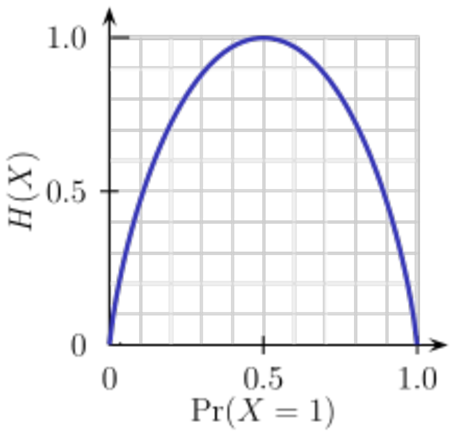
\includegraphics[scale=0.75]{entropia} 
\end{center}
\caption{Representación gráfica de h(x)}
\label{fig:hx}
\end{figure}

\end{frame} 

%%%%%%%%%%%%%%%%%%%%%%%%%%%%%%%%
\subsection{Incertidumbre}

\begin{frame}  \frametitle{Incertidumbre}\small

\begin{itemize}
\item Una  posible interpretación que nos proporciona la representación gráfica es que la entropía es una medida de \textbf{incertidumbre}. 


\item La mayor incertidumbre sobre cual símbolo es emitido ocurre cuando dos símbolos son igualmente probables $(x=\frac{1}{2})$, por otro lado no existe incertidumbre si ninguno de los símbolos son emitidos (x=0 ó x=1). 

\item A modo de resumen, podemos establecer que la entropía es una medida de incertidumbre sobre la identidad del símbolo que es obtenido acorde con una distribución de probabilidad \textbf{p}. 





\end{itemize}

\end{frame} 

%%%%%%%%%%%%%%%%%%%%%%%%%%%%%%%%
\begin{frame}  \small


El concepto de información está muy vinculado a la incertidumbre. Básicamente, proporcionar información sobre un evento reduce nuestra incertidumbre sobre él. 


\begin{teorema}[El teorema de comparación]
Si $p_1, p_2, \ldots , p_m$ y $q_1, q_2, \ldots , q_m$ son dos distribuciones de probabilidad entonces:

\begin{center}
$H_b(p) =  \sum^{m}_{i=1} p_i log_b(\frac{1}{p_i}) \leq \sum^{m}_{i=1} p_i log_b(\frac{1}{q_i}) $
\end{center}

El caso de igualdad es dado sii $q_i=p_i$ para todos los i $(1\leq i \leq m)$.

\end{teorema}



\begin{teorema}
La entropía (incertidumbre) de una distribución p en m símbolos es al menos $log_b m$. 
El máximo valor ocurre sii todos los símbolos son equiprobables.
\end{teorema}


\end{frame} 

%%%%%%%%%%%%%%%%%%%%%%%%%%%%%%%%
\begin{frame}  \small

\begin{ejercicio}
Suponemos una fuente sin memoria que emite tres símbolos a,b,c con probabilidades 0.6, 0.3, 0.1, y otra fuente sin memoria emite los mismos símbolos, con probabilidades 0.5, 0.3, 0.2. ¿Qué fuente presenta mayor incertidumbre? ¿Qué distribución de probabilidad produciría la mayor incertidumbre?
\end{ejercicio}

\pause

\underline{\textbf{Solución}}:\\

a) $H_2(p) = 0.6 log_2(1/0.6) + 0.3 log_2(1/0.3) + 0.1 log_2(1/0.1)$\\
   $ = 0.6 \times 0.74 +  0.3 \times 1.73 + 0.1 \times 3.32$\\
   $ = 0,44 +0,52 + 0,33 =  1.29 $ \\

b) $H_2(p) =  0.5 log_2(1/0.5) + 0.3 log_2(1/0.3) + 0.2 log_2(1/0.2)$\\
	$ = 0.5 +  0.3 x 1.73 + 0.2 x 2.32 = 0,5 +0,52 + 0,46$
	$=  1.48 $\\

c)  La incertidumbre es mayor cuando todos los símbolos son igualmente probable, siendo la distribución de probabilidad $(\frac{1}{3},\frac{1}{3},\frac{1}{3})$. $H_2(p) = log_2(m=3) = 1,58.  $\\

\end{frame} 

\subsection{Códigos Óptimos}
%%%%%%%%%%%%%%%%%%%%%%%%%%%%%%%%
\begin{frame}  \frametitle{Códigos Óptimos}\small

\begin{itemize}
\item Después de las definiciones planteadas, volvemos a una pregunta que teníamos sin resolver: ¿Cómo encontrar un código b-ario UD para una fuente (S,p) tal que la  longitud media de palabra  L es mínima? . 

\item Para realizarlo hacemos uso del concepto de entropía $H_b(p)$ y los siguientes teoremas:

\end{itemize}

\begin{teorema}
La longitud media de cualquier código UD b-ario para la fuente (S,p) verifica $L \geq H_b(p).$


\begin{center}

El límite inferior de L está definido por la entropía.
\vspace{0.25cm}

$L=p_1y_1+p_2y_2+ \ldots +p_my_m$ \hspace{0.25cm} \geq \hspace{0.25cm}
$H_b(p) =  \sum^{m}_{i=1} p_i log_b(\frac{1}{p_i})  $
\end{center}

\end{teorema}

\end{frame} 
%%%%%%%%%%%%%%%%%%%%%%%%%%%%%%%%
\begin{frame}  \small

\begin{definicion}[Regla de Shannon-Fano (SF)]

Podemos intentar construir un código con una media de longitud de palabra cercana a L.
\vspace{0.25cm}\\
Partiendo del Teorema 3. 

\begin{center}
$L=p_1y_1+p_2y_2+ \ldots +p_my_m$ \hspace{0.25cm} \geq \hspace{0.25cm}
$H_b(p) =  \sum^{m}_{i=1} p_i log_b(\frac{1}{p_i})  $

\end{center}

\begin{center}Por ejemplo: 
$ p_1 y_1 \geq p_1 log_b(\frac{1}{p_1})  \rightarrow  $ 
$  y_1 \geq log_b(\frac{1}{p_1})  \rightarrow  b^{y_1} \geq \frac{1}{p_1}  $
\end{center}

escogiendo $b^{y_{i}}$ sea tan cercano como sea posible a $\frac{1}{p_i}$.

O lo que es lo mismo, ya que son bits (debe de ser entero):

\begin{center}
$y_i$ es el menor entero positivo tal que $b^{y_{i}}  \geq \frac{1}{p_i}.$
\end{center}

El valor resultante de K es:

\begin{center}
$ K= 1/b^{y_{1}}+1/b^{y_{2}}+\ldots+1/b^{y_{m}} \leq p_1+p_2+\ldots+p_m=1$
\end{center}

y por tanto un código PF (por teorema 2.2) con estos parámetros debe existir.

\end{definicion}


\end{frame} 


%%%%%%%%%%%%%%%%%%%%%%%%%%%%%%%%
\begin{frame}  \small

El siguiente teorema muestra que la longitud media L de un código esta muy próxima a $H_b(p)$ y define la cota superior.

\vspace{1cm}
\begin{teorema}\label{theorem:limitemenor}
Existe un código PF b-ario para una fuente con una probabilidad de distribución \textbf{p} que verifica la inegualdad  $L < H_b(p) + 1$.	
\end{teorema}

\end{frame} 
%%%%%%%%%%%%%%%%%%%%%%%%%%%%%%%%

%%%%%%%%%%%%%%%%%%%%%%%%%%%%%%%%
\begin{frame}  \small

\begin{ejemplo}

Una fuente emite 5 símbolos con una probabilidad de distribución $p = [0.4, 0.2, 0.2, 0.1, 0.1]$.
¿Cual es la entropía H(p)? Construya un código binario para esta fuente con longitud media de palabra menor que $H(p) + 1$.\\
\end{ejemplo}

\pause

\textit{\underline{Solución}}:\\
	Utilizamos el hecho que H(p) es la entropía con respecto a la base b = 2. Un simple cálculo muestra que $H(p) \approx 2.12$. 
	
\begin{center}
$H_2(p)	=  0.4 \times log_2(\frac{1}{0.4})+ 0.2 \times log_2(\frac{1}{0.2})$ + $0.2 \times log_2(\frac{1}{0.2}) + 0.1 \times log_2(\frac{1}{0.1}) + 0.1 \times log_2(\frac{1}{0.1}) =2.12$
\end{center}

La regla SF nos indica que debemos escoger $y_1$ el menor entero que cumpla

\begin{center}
$2^{y_{1}} \geq \frac{1}{0.4} = 2.5$
\end{center}

cuyo resultado es, $\mathbf {y_1} = 2$.  



\end{frame} 
%%%%%%%%%%%%%%%%%%%%%%%%%%%%%%%%

%%%%%%%%%%%%%%%%%%%%%%%%%%%%%%%%
\begin{frame}  \small

De forma similar podemos calcular los demás casos:

\begin{center}
$\mathbf {y_2} = 3$ \tiny{$(2^{y_{2}} \geq \frac{1}{0.2} = 5)$}, \small $\,\, \mathbf {y_3} = 3$ \tiny $(2^{y_{3}} \geq \frac{1}{0.2} = 5)$,\\
\vspace{0.25cm}
\small $\mathbf {y_4} = 4$  \tiny $(2^{y_{4}} \geq \frac{1}{0.1} = 10),$\small $ \,\, \mathbf {y_5} = 4 $  \tiny  $(2^{y_{5}} \geq \frac{1}{0.1} = 10).$
\end{center}

Por tanto,  ($n_i=$ Número $(y_j = i)$) los parámetros requeridos son $n_2 = 1,n_3 = 2,n_4 = 2$. 

\vspace{0.5cm}

Utilizando el método del árbol, es fácil construir un código PF con esos parámetros, por ejemplo: 

\begin{center}
 00, 010, 011, 1000, 1001.
\end{center}	

El tamaño medio sería: 

\begin{center}
L = 0.4 x 2 + 0.2 x 3 + 0.2 x 3 + 0.1 x 4 + 0.1 x 4 = 2.8,
\end{center}

que verifica (como garantiza el teorema \ref{theorem:limitemenor}) que es menor que $H(p) + 1$ $\approx 3.12.$

\end{frame} 
%%%%%%%%%%%%%%%%%%%%%%%%%%%%%%%%

%%%%%%%%%%%%%%%%%%%%%%%%%%%%%%%%
\begin{frame}  \small

\begin{ejercicio}\label{ej:SF}

Utiliza la regla de codificación Shannon-Fano para construir un código binario PF para una fuente con una distribución de probabilidad p = [0.25, 0.10, 0.15, 0.05, 0.20, 0.25]. Encuentra la longitud media de palabra L, y verificar que L está ente  H(p) y H(p) + 1.

\end{ejercicio}
\pause

\textit{\underline{Solución}}:\\
\footnotesize

$H_2(p)	=  0.25 \times log_2(\frac{1}{0.25})+ 0.1 \times log_2(\frac{1}{0.1})$ + $0.15 \times log_2(\frac{1}{0.15}) + 0.05 \times log_2(\frac{1}{0.05}) + 0.2 \times log_2(\frac{1}{0.2}) + 0.25 \times log_2(\frac{1}{0.25}) =2.42$\\


\begin{center}
$2^{y_{1}} \geq \frac{1}{0.25} = 4; y_{1} =2$  $2^{y_{2}} \geq \frac{1}{0.1} = 10; y_{2} =4$
\end{center}
\begin{center}
$2^{y_{3}} \geq \frac{1}{0.15} = 6.66; y_{3} =3$  $2^{y_{4}} \geq \frac{1}{0.05} = 20; y_{4} =5$
\end{center}
\begin{center}
$2^{y_{5}} \geq \frac{1}{0.2} = 5; y_{5} =3$ $2^{y_{6}} \geq \frac{1}{0.25} = 4; y_{6} =2$
\end{center}

$n_2 = 2,n_3 = 2,n_4 = 1,n_5 = 1$. \\

\begin{center}
L = 0.25 x 2 + 0.25 x 2 + 0.20 x 3 + 0.15 x 3 + 0.10 x 4 + 0.05 x 5= 2.7.
\end{center}

Verifica que $2.42\leq 2.7 \leq 3.42$.

\end{frame} 

%%%%%%%%%%%%%%%%%%%%%%%%%%%%%%%%
\begin{frame}  \small

\begin{ejercicio}

Utiliza la regla de codificación Shannon-Fano para construir un código ternario PF para una fuente con una probabilidad de distribución 
p = [0.5,0.3,0.2]. Muestra, construyendo un código mejor que este código no es óptimo.
\end{ejercicio}
\pause

\textit{\underline{Solución}}:\\

$H_3(p)	=  0.5 \times log_3(\frac{1}{0.5})+ 0.3 \times log_3(\frac{1}{0.3})$ + $0.2 \times log_3(\frac{1}{0.2})  =0.93$\\

\begin{center}
$3^{y_{1}} \geq \frac{1}{0.5} = 2; \mathbf {y_{1}} =1$  $3^{y_{2}} \geq \frac{1}{0.3} = 3.33; \mathbf{y_{2}} =2$ $3^{y_{3}} \geq \frac{1}{0.2} = 5;\mathbf { y_{3} }=2$  \\
\vspace{0.25cm}
$n_1 = 1,n_2 = 2$. \\
\end{center}

\begin{center}
L = 0.5 x 1 + 0.3 x 2 + 0.2 x 2 = 1.5.
\end{center}

Verifica que $0.93 \leq 1.7 \leq 1.93$.

\vspace{0.25cm}
\color{red}{Pero podríamos crear un código con 1 bit cada uno}:
\begin{center}
L = 0.5 x 1 + 0.3 x 1 + 0.2 x 1 = 1.
\end{center}

\end{frame} 

%%%%%%%%%%%%%%%%%%%%%%%%%%%%%%%%
%%SECTION          %%%%%%%%%%%%%%%%%%%
%%%%%%%%%%%%%%%%%%%%%%%%%%%%%%%%
%%%%%%%%%%%%%%%%%%%%%%%%%%%%%%%%
%%%%%%%%%%%%%%%%%%%%%%%%%%%%%%%%
%%%%%%%%%%%%%%%%%%%%%%%%%%%%%%%%
\section{Regla de Huffman}
%%%%%%%%%%%%%%%%%%%%%%%%%%%%%%%%
\begin{frame}  \frametitle{Regla de Huffman}\footnotesize 

\begin{itemize}
\item Si un código UD existe, entonces es posible construir un código PF con los mismos parámetros. Por tanto, debemos restringir la búsqueda de códigos óptimos a códigos que cumpla la propiedad PF.

\item La regla de Shannon-Fano produce códigos satisfactorios, pero por regla general no nos ofrece un código óptimo.

\item  La regla de Huffman, descrita a continuación, nos garantiza un código óptimo. (regla similar puede ser para $b > 2$.)
 \end{itemize}

\begin{lema}
Un código óptimo PF $c: S\rightarrow \mathbb{B}^{*}$ para una fuente (S,p) tiene las siguientes propiedades:
\begin{enumerate}
\item si la palabra codificada c(s') es mayor que c(s) entonces $p_s \geq p_s'$
\item entre las palabras codificadas de máxima longitud hay dos de la siguiente forma x0 y x1, para algún $x  \in \mathbb{B}^{*}$
\end{enumerate}
\end{lema}


\end{frame} 

%%%%%%%%%%%%%%%%%%%%%%%%%%%%%%%%
\begin{frame}  \small

La regla de Huffman emplea dos construcciones basadas en estas propiedades:

\begin{description}
\item[H1] Dada una fuente (S,p), sea s' y s'' dos símbolos con las menores probabilidades. Construir una nueva fuente $(S^{*},p^{*})$  remplazando s' y s'' por un símbolo $s^{*}$, con probabilidad $p^{*}_{s*}= p_{s'}+p_{s''}$. Todos los demás símbolos se mantienen con las mismas probabilidades.

\item[H2] Si tenemos un código binario $ h^{*} $ para $ (S^{*},p^{*}) $ con $ h^{*}(s^{*}) =w$, entonces definimos un código binario PF h para (S,p) mediante las reglas $h(s')=w0$, $h(s'')=w1$, y $h(u) = h^{*}(u)$ para todos $ u \neq	s',s''$.
\end{description}

\end{frame} 
%%%%%%%%%%%%%%%%%%%%%%%%%%%%%%%%
\begin{frame}  \small

\begin{figure}[!hbtp]
\begin{center}
	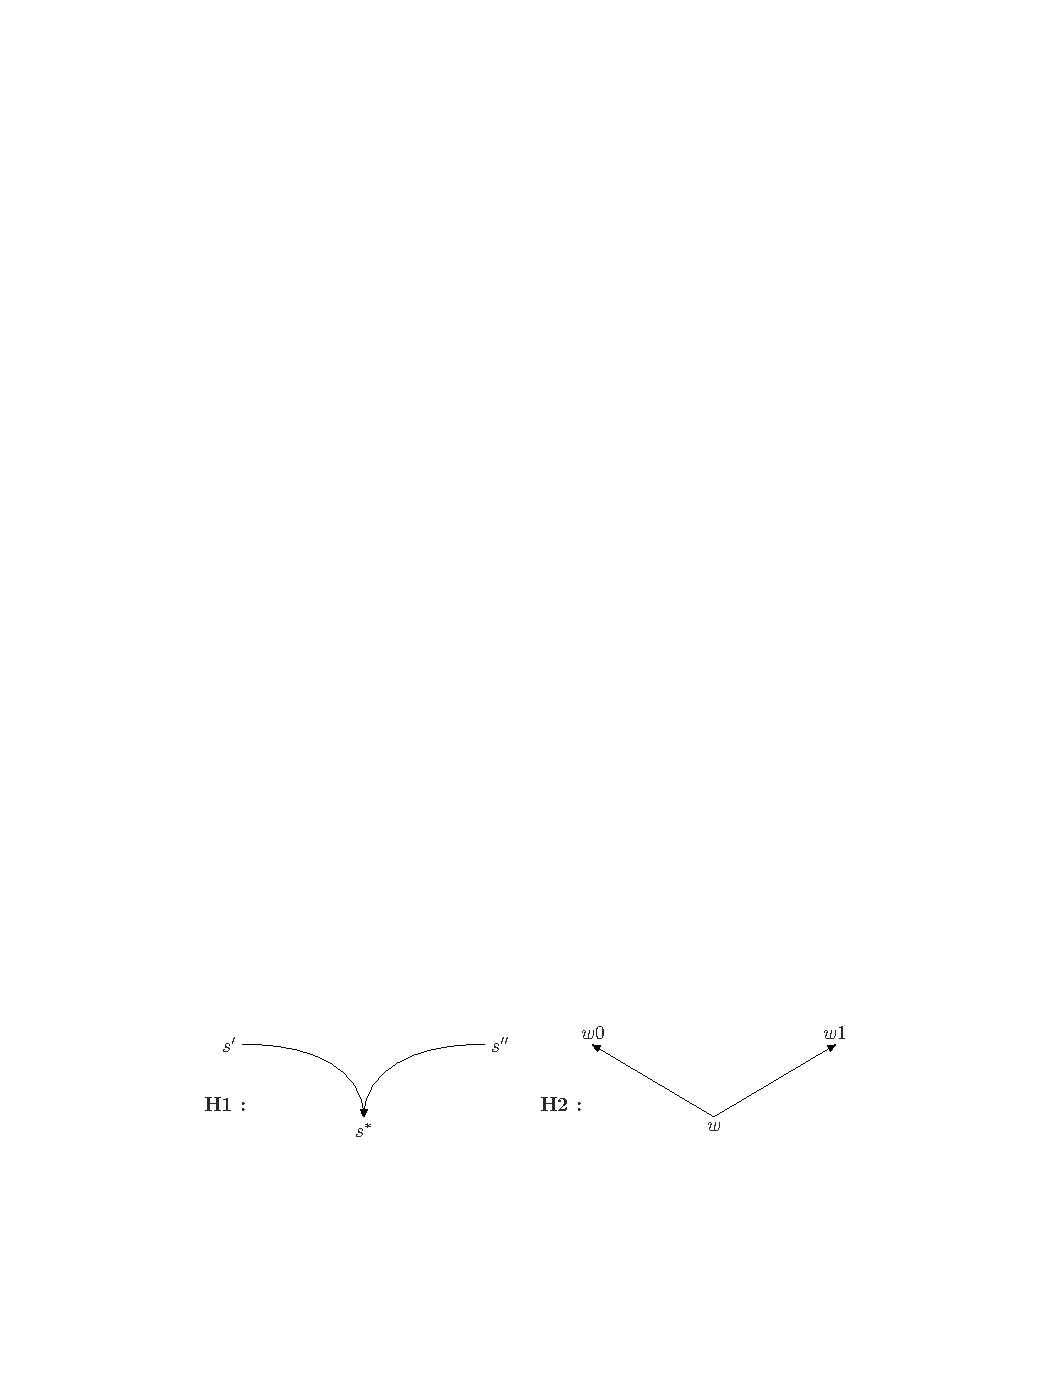
\includegraphics[scale=0.75]{Huffman} 
\end{center}
\caption{Las dos reglas de Huffman}
\label{fig:huffman}
\end{figure}

\begin{itemize}\footnotesize 
\item Supongamos que tenemos una fuente con m símbolos. 

\item La regla H1 puede ser utilizada para construir una secuencia de fuentes cada una con un símbolo menos que la anterior, por lo que el proceso finalizaría en la fuente m\textit{th}, la cual solamente posee un símbolo. 

\item El código óptimo para la última fuente es la asignación de la palabra vacía a ese símbolo único. 

\item Una vez aplicado lo anterior, la H2 puede ser utilizada para construir los códigos para cada una de las fuentes en la secuencia. 
\end{itemize}




%La optimalidad de los códigos resultantes será retomada posteriormente.


\end{frame} 
%%%%%%%%%%%%%%%%%%%%%%%%%%%%%%%%
\begin{frame}  \small
\begin{ejemplo}
Utilizar la regla de Huffman para construir un código optimo para una fuente con distribución p = [0.4, 0.2, 0.2, 0.1, 0.1].\\
\end{ejemplo}

\pause

\textit{\underline{Solución}}:\\
Comenzando con $p^{(1)} = p$ y definiendo $p^{(i+1)} = p^{(i)*}$ para i = 1, 2, 3, 4, la regla H1 produce la secuencia de fuentes mostrada en la siguiente figura.

\begin{figure}[!hbtp]
\begin{center}
	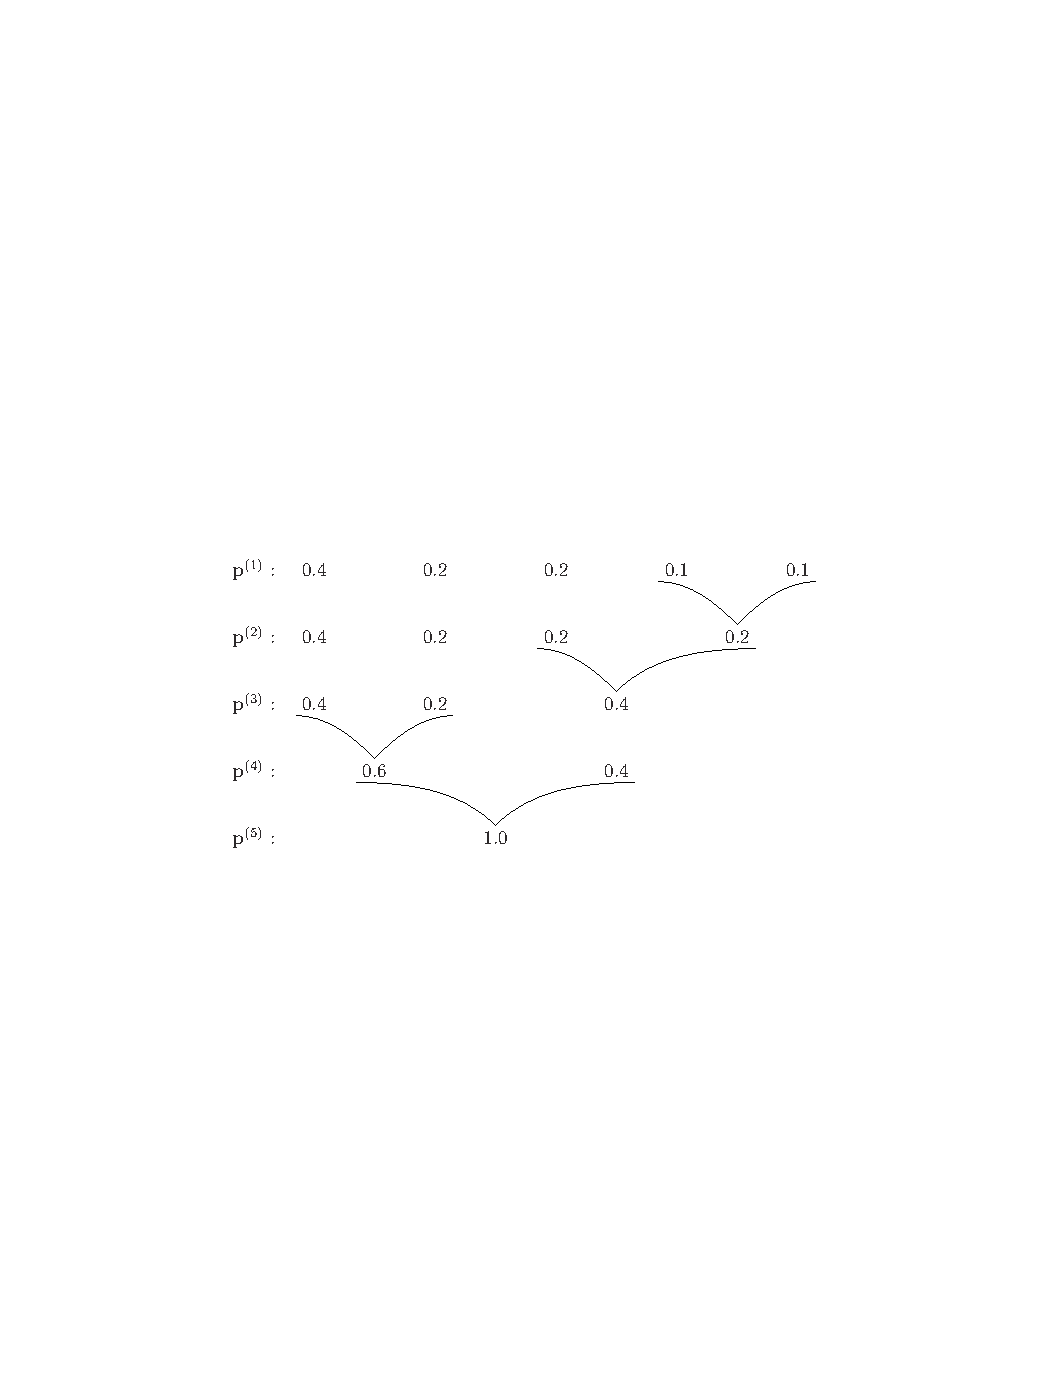
\includegraphics[scale=0.5]{H1} 
\end{center}
\caption{Aplicación regla H1 Huffman}
\label{fig:h1}
\end{figure}




\end{frame} 
%%%%%%%%%%%%%%%%%%%%%%%%%%%%%%%%
\begin{frame}  \small

Para construir el código Huffman utilizamos la H2, comenzando del código que asigna la palabra vacía al símbolo único en la última fila. El proceso es mostrado en la siguiente figura. 

\begin{figure}[!hbtp]
\begin{center}
	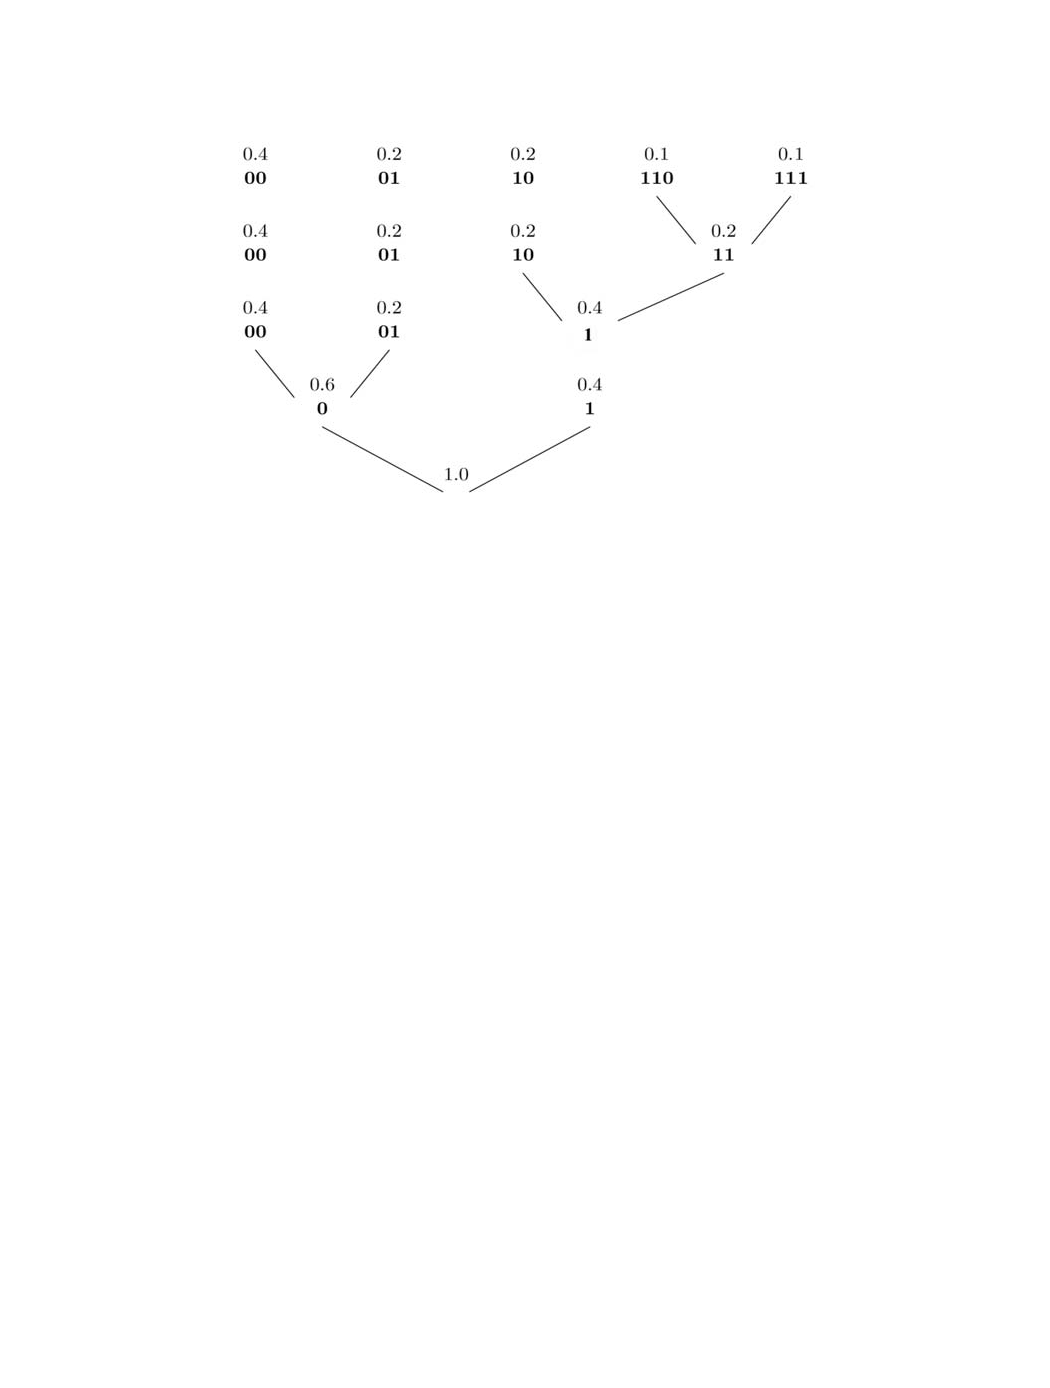
\includegraphics[scale=0.6]{H2} 
\end{center}
\caption{Aplicación regla H2 Huffman}
\label{fig:h2}
\end{figure}

\end{frame} 


%%%%%%%%%%%%%%%%%%%%%%%%%%%%%%%%

%%%%%%%%%%%%%%%%%%%%%%%%%%%%%%%%
\begin{frame}  \small

\begin{itemize}
\item Las palabras codificadas son 00, 01, 10, 110, 111. 
\item Para esta fuente la longitud media de palabra del código Huffman es:
\begin{center}
$L_{opt}=(0.4+0.2+0.2) \times 2 + (0.1+0.1) \times 3=2.2$
\end{center}

\item La entropía H = H(p) es aproximadamente 2.12. 

\item En el ejemplo anterior aplicando la regla SF a esta fuente obteniendo un código con una media de longitud de palabra de $L_{SF} = 2.8$.

\item La relación entre los resultados obtenidos con la regla de huffman y los obtenidos anteriormente es: 
\begin{center}
$H < L_{opt}< L_{SF} < H+1.$
\end{center}

\end{itemize}

\end{frame} 

%%%%%%%%%%%%%%%%%%%%%%%%%%%%%%%%
%\begin{frame} \small

%\begin{lema}
%Sea h y $h^{*}$ definidas como en la regla H2. Entonces la longitud media de palabras de h y $h^{*}$  satisfacen 
%\begin{center}
%$L(h) = L(h^{*}) + p^{*}_{s^{*}}$ 
%\end{center}
%\end{lema}

%\begin{teorema}
%Si  $ h^{*} $ es óptimo para $(S^{*}, p^{*})$ entonces h es óptimo para (S, \textbf{p}).
%\end{teorema}

%\end{frame} 

%%%%%%%%%%%%%%%%%%%%%%%%%%%%%%%%
\begin{frame}  \small

\begin{ejercicio}
Construya un código óptimo para la fuente del Ejercicio \ref{ej:SF} utilizando la regla de Huffman, y calcule su longitud media de palabra.
\end{ejercicio}

\begin{ejercicio}
Considere una fuente con probabilidad de distribución [0.4,0.3,0.2,0.1]. Compare la longitud media de palabra del código obtenido de la regla SF con la longitud media de palabra óptima obtenida mediante la regla de Huffman.
\end{ejercicio}

%Suppose that seven symbols are emitted by a source, with probability distribution p = [0.2,0.2,0.2,0.1,0.1,0.1,0.1]. What is the entropy of the source?
%Use the Shannon-Fano rule to construct a prefix-free code for this source. Find its average word-length L, and verify that Theorems 3.10 and 3.12 hold. Use Huffman’s rule to construct an optimal bi- nary code for this source.


\end{frame} 
%%%%%%%%%%%%%%%%%%%%%%%%%%%%%%%%
%%%%%%%%%%%%%%%%%%%%%%%%%%%%%%%%
%SECCION %%%%%%%%%%%%%%%%%%%%%%%%%%%%%%%
%%%%%%%%%%%%%%%%%%%%%%%%%%%%%%%%
%%%%%%%%%%%%%%%%%%%%%% 

%%%%%%%%%%%%%%%%%%%%%%%%%%%%%%%%
%%%%%%%%%%%%%%%%%%%%%%%%%%%%%%%%
%\begin{frame}  \small \begin{ejercicio} \end{ejercicio} \pause \textit{\underline{Solución}}:\\ \end{frame} 
%%%%%%%%%%%%%%%%%%%%%%%%%%%%%%%%
%%%%%%%%%%%%%%%%%%%%%%%%%%%%%%%%
%EJERCICIO %%%%%%%%%%%%%%%%%%%%%%%%%%%%%%%
%%%%%%%%%%%%%%%%%%%%%%%%%%%%%%%%

%%%%%%%%%%%%%%%%%%%%%%%%%%%%%%%%
%\begin{frame}  \small  
%\begin{itemize} \item  \item \item \item 
%\end{itemize} \end{frame} 

%%%%%%%%%%%%%%%%%%%%%%%%%%%%%%%%
%\begin{frame}  \small  
%\end{frame} 





\begin{frame} %\frametitle{Preguntas}

%\begin{center}
%¡Gracias por su atención!\\
%\end{center}
\vspace*{2cm}

\begin{center}
\textbf{José A. Montenegro Montes} \\

\textit{Dpto. Lenguajes y Ciencias de la Computación}\\
\textit{ETSI  Informática. Universidad de Málaga}\\
\textbf{jmmontes@uma.es}\\
%\href{https://twitter.com//monteDocencia}{
%
\includegraphics[height=0.05\textheight]{twitter.jpg}}
\end{center}

\vspace*{1,5cm}


\includegraphics[height=0.15\textheight]{logoUma.jpg} \hspace*{3.6cm}

\includegraphics[height=0.15\textheight]{logoInf.jpg}   \hspace*{3.7cm}

\includegraphics[height=0.15\textheight]{logoLcc.jpg}  




\end{frame} 

\end{document} 